\section{Module system}
\label{sec:dai_modules}

\todo{Assigned Jakob}

The module system of Hopper is designed to be simple to implement.

Hierarchical module names are supported, e.g. \texttt{A.B.C}. Only a single source directory is supported, so there is a straight-forward translation from module names to file paths: the above example maps to \texttt{A/B/C.hpr}. This restriction removes the possibility of conflicts where multiple matching source files exist in different source directories.

\subsection{Dependency model}
Modules explicitly declare what functions and data types they export, and declare dependency on other modules using \texttt{import} statements. Importing a module means importing \emph{everything} that module exports, so fully qualified names are required when referring to imported functions or data types. For example, if module \texttt{A} defines a function \texttt{f} which module \texttt{B} wishes to use, module \texttt{B} must first \texttt{import A} and then use the notation \texttt{A.f} whenever it wants to use \texttt{f}. This ensures that imported functions do not cause name clashes.

The import statements are used to build a \gls{dag} representing the dependency relations of the program. Verifying that the graph actually is acyclic ensures that no cyclical dependencies occur. \glslink{topsort}{Topologically sorting} the nodes of the \gls{dag} gives a compilation order where the dependencies of each module are compiled before that module. This design ensures that type information for a module's imports is available at compile time, so that the compiler only has to consider a single module at a time. For example, the module hierarchy in Figure~\ref{fig:depgraph} yields a compile order of D, B, E, C, A.

\begin{figure}[h!]
\centering
  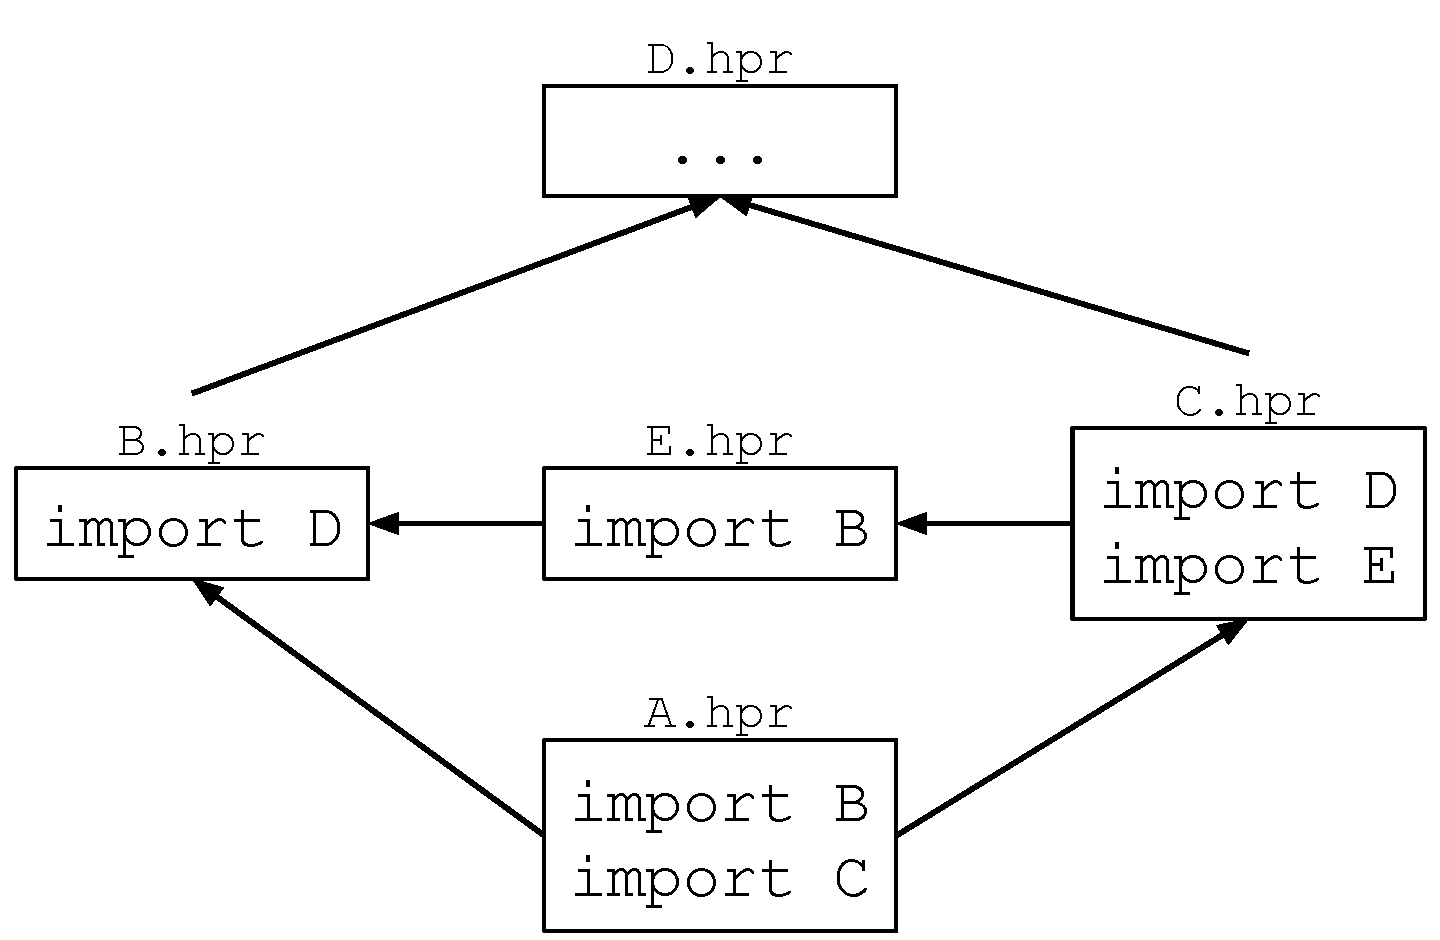
\includegraphics[width=0.6\pdfpagewidth]{figure/depgraph}
  \caption{Example dependency graph}
  \label{fig:depgraph}
\end{figure}

\subsection{Interface files}
In order to propagate type information for a given module's exports into the modules that depend on it, the concept of \texttt{.hip} interface files is used. Hopper's interface files are similar in concept to those of Haskell's\cite{interfacefiles}, but much more basic. They contain maps from identifiers to type information (which might have been given explicitly, or inferred by the type checker) for everything that is exported from a given module, and are written by the type checker after a successful run.

The actual implementation of the interface files simply uses derived \texttt{Show} and \texttt{Read} instances for the data types representing Hopper types.